We are also interested in the impacts of different traffic patterns on scaling
performance. As such, we send our test web server application web requests in a
variety of patterns and examine which traffic pattern the scaling method handles
well, and which traffic pattern the scaling method does not handle well.
Moreover, we also examine scaling methods in relation to each other with respect
to different traffic patterns, seeking to answer for which traffic patterns
predictive auto-scaling is beneficial and which traffic patterns predictive
auto-scaling is detrimental or meaningless.

In this thesis we examine four different traffic patterns that we feel are
fairly indicative of the different traffic patterns a web application may face.
We entitle these patterns \textit{step-ladder}, \textit{jagged-edge},
\textit{increase-decrease}, and
\textit{flash-crowd}.\footnote{There are of course an infinite number of traffic
patterns that we could examine, and examining other options is an exciting
opportunity for future work.} We describe each of these patterns, and offer a
visual representation for each, below. Each pattern runs for at least twenty
minutes and at most forty minutes, and makes at most 20 requests per second.\footnote{All
traffic patterns have a start and end buffer at which they receive
only 1 request per second, to ensure we do not immediately overload the
application.} These values were chosen to give
space for the lengthier pod initialization times and to keep the network from
becoming too congested respectively. We can imagine the all traffic seen by a
typical web server as being composed of different combinations of these patterns
across longer time spans.

\begin{itemize}
  \item \textbf{step-ladder}: The traffic pattern \textit{step-ladder}, visible
    in Figure \ref{fig:step-ladder}, represents a web server which faces a load
    pattern which increases immediately at predicted intervals. This scenario
    can be seen as representing, for example, an video streaming website which
    experiences predictable increases in traffic as different shows are
    streamed. This traffic pattern begins with 1 request per second for 3
    minutes, before immediately increasing to 4 requests per second. The process
    of increasing by 3 requests per second and then staying constant for 3
    minutes continues for 6 more iterations until it reaches 19 requests per
    second.

    \begin{figure}[!h]
      \centerline{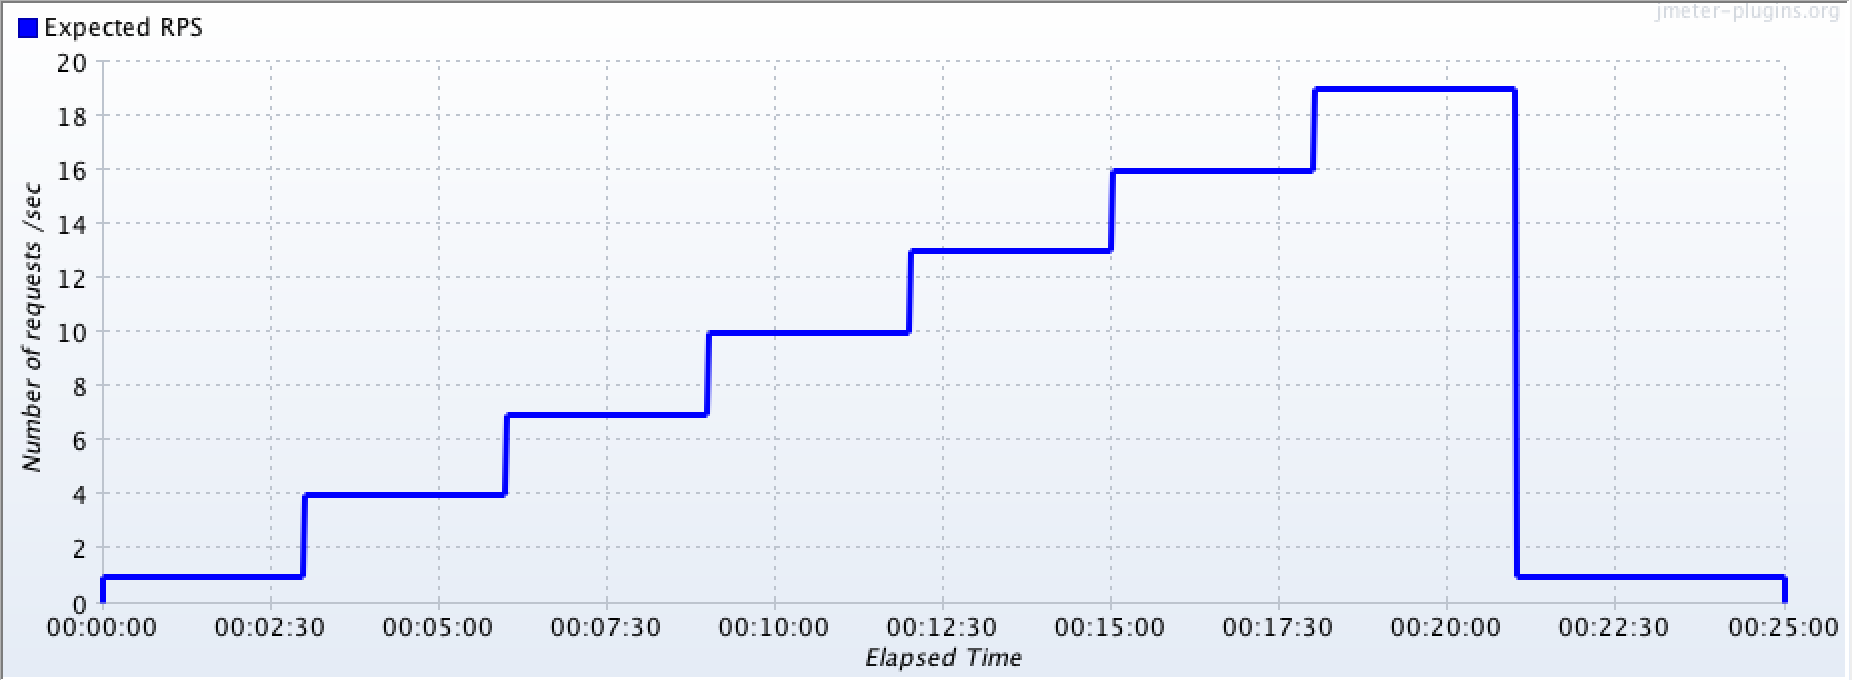
\includegraphics[scale=.4]{step-ladder.jpg}}
      \caption{The step-ladder Traffic Pattern.}
      \label{fig:step-ladder}
    \end{figure}

  \item \textbf{jagged-edge}: The traffic pattern \textit{jagged-edge}, visible
    in Figure \ref{fig:jagged-edge}, is similar to \textit{step-ladder},
    although it reflects a more gradual increase and decrease in load. Thus, it
    applies to a similar scenario as \textit{step-ladder}. It begins at 1
    request per second for 3 minutes before increasing to 10 requests per
    second over the course of 5 minutes. It then decreases to 5 requests per
    second over the course of 2 minutes. This pattern of increasing by 10
    requests per second over the course of 5 minutes and then decreasing by 5
    requests per second over the course of 2 minutes continues until reaching 20
    requests per second, and which point we transition to the end buffer period
    of 1 request per second for 5 minutes.

    \begin{figure}[!h]
      \centerline{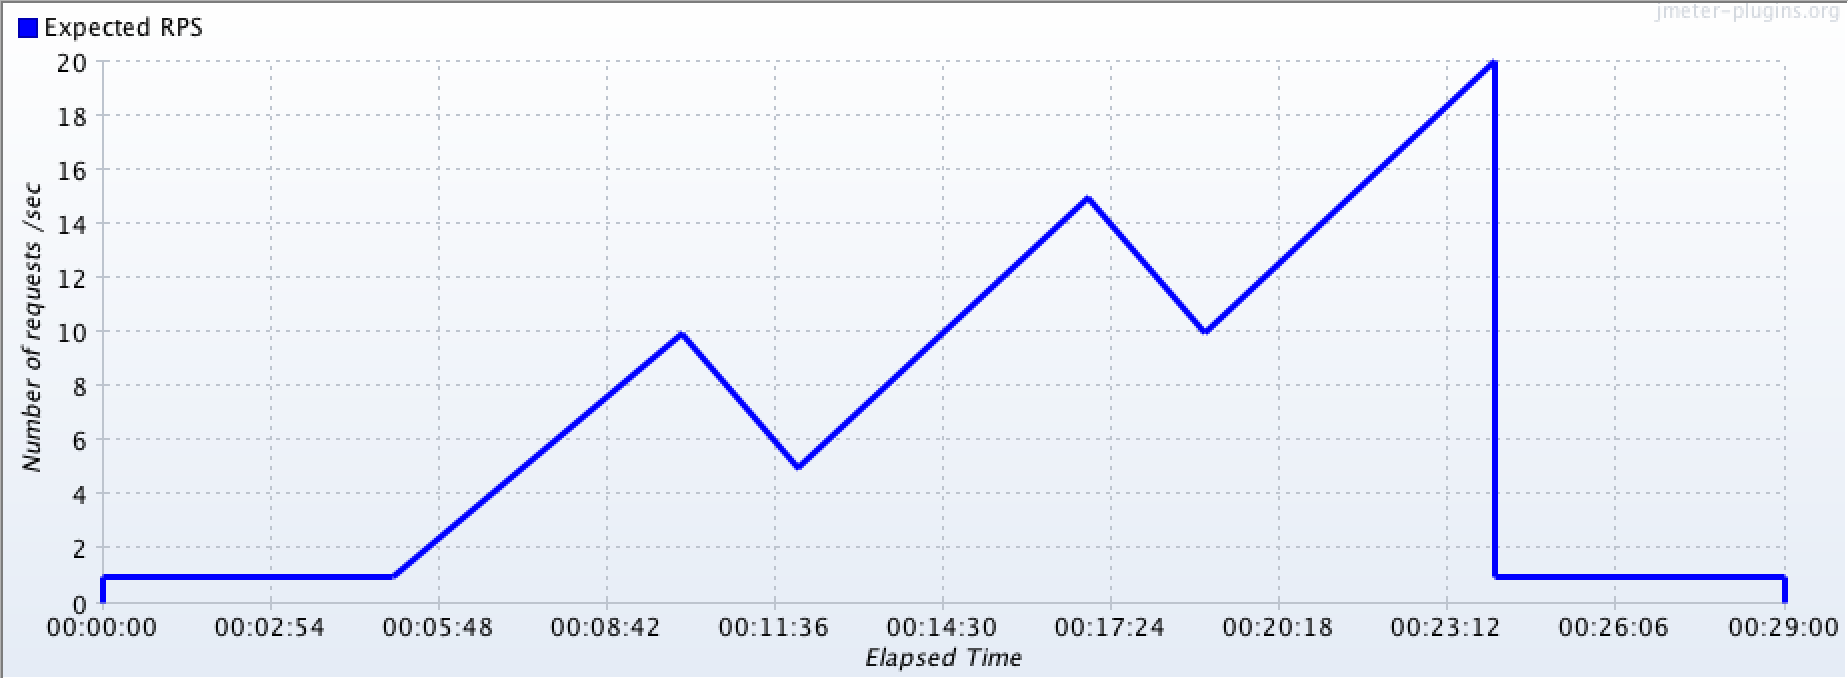
\includegraphics[scale=.4]{jagged-edge.jpg}}
      \caption{The jagged-edge Traffic Pattern.}
      \label{fig:jagged-edge}
    \end{figure}

  \item \textbf{increase-decrease}: The traffic pattern
    \textit{increase-decrease}, visible in Figure \ref{fig:increase-decrease},
    represents a web server facing constantly increasing and then constantly
    decreasing load. This scenario can be seen as representing, for example, a
    restaurant in which people increasingly visit the site as it becomes closer
    and closer to a meal time, and decreasingly visit the site as a meal time
    becomes farther and farther away. After five minutes of initialization at
    1 request per second, our load
    generator builds from sending 1 request per second to 20 requests per
    second over the course of 15 minutes. After reaching the apex, the traffic
    generator then reduces from sending 20 requests per seconds to sending 1
    request per second, again over the course of 15 minutes.

    \begin{figure}[!h]
      \centerline{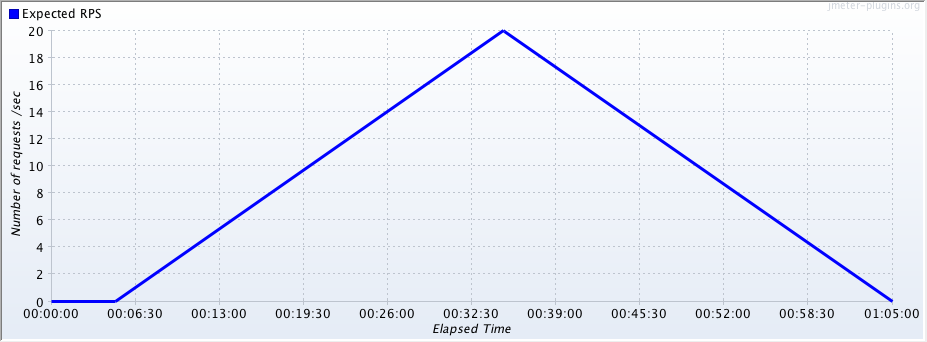
\includegraphics[scale=.4]{increase-decrease.jpg}}
      \caption{The increase-decrease Traffic Pattern.}
      \label{fig:increase-decrease}
    \end{figure}

  \item \textbf{flash-crowd}: The traffic pattern \textit{flash-crowd}, visible
    in Figure \ref{fig:flash-crowd}, represents a web server facing a suddenly
    increasing, and then suddenly decreasing, amount of load. This scenario is
    indicative of, for example, a news website which suddenly receives a
    short-lived burst of traffic when a major story hits. After five minutes of
    sending 1 request per second, our load generator
    builds from sending 1 request per second
    to sending 5 requests per second, over the course of 5 minutes. Then, in
    just 2 minutes, our load generator jumps from sending 5 requests per second
    to sending 20 requests per second. After reaching the apex, the traffic
    generator decreases from sending 20 requests per second to sending 5
    requests per second, again in just 2 minutes. Finally, our load generator
    decreases from sending 5 requests per second to 1 request per second, over
    the course of 5 minutes, before transitioning to the end buffer period of 1
    request per second for 5 minutes.

    %% We use flash-crowd-short although we refer to it as flash-crowd.
    \begin{figure}[!h]
      \centerline{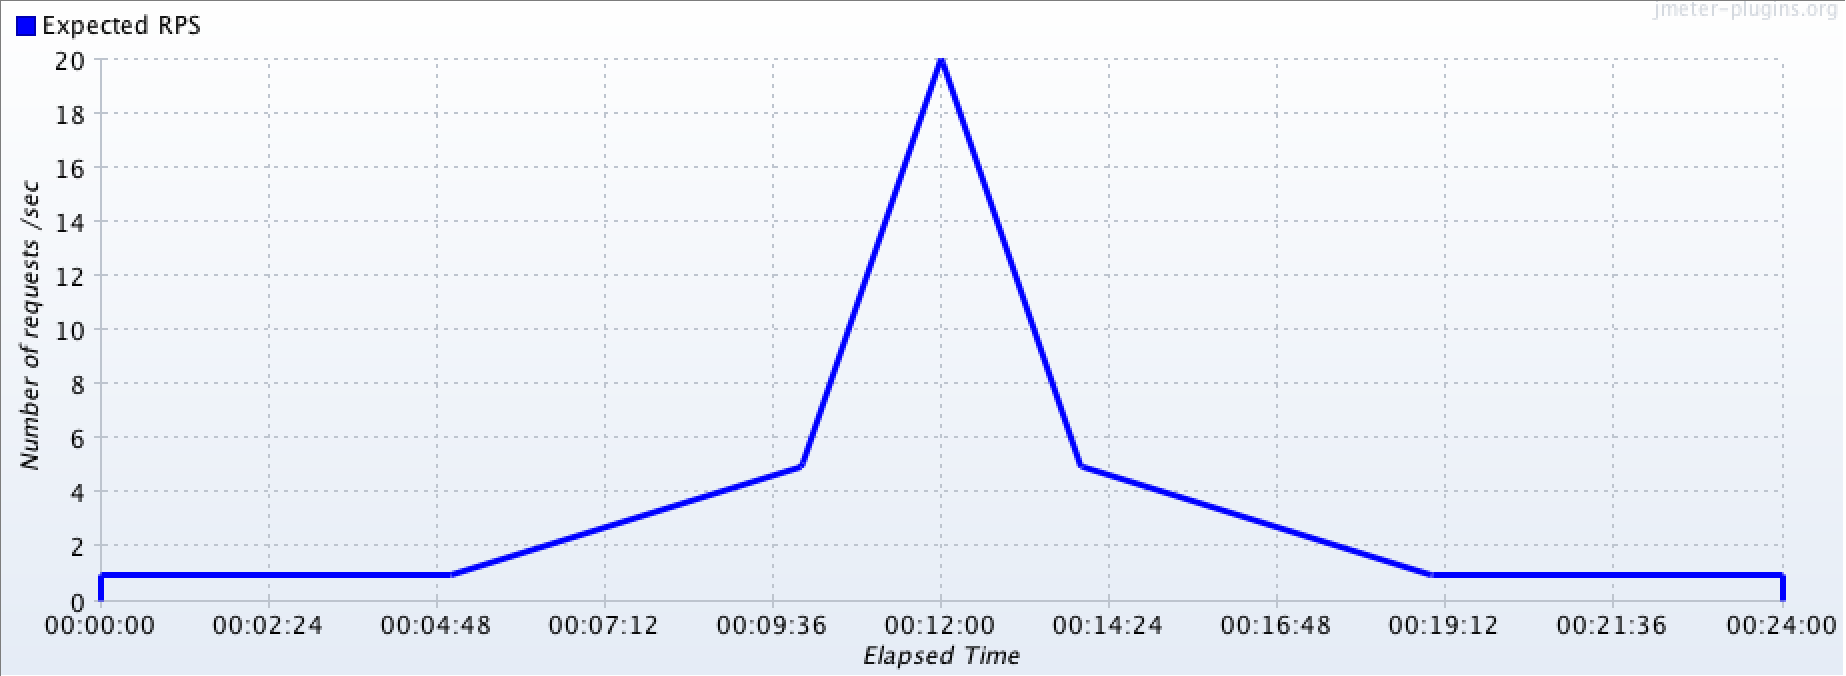
\includegraphics[scale=.4]{flash-crowd-short.jpg}}
      \caption{The flash-crowd Traffic Pattern.}
      \label{fig:flash-crowd}
    \end{figure}

\end{itemize}
